\Exhibit{PubScoring}{%
    Справочная страница pub.dev, объясняющая рейтингование пакетов%
}

На этой странице говорится:

\begin{itemize}

    \item \Quote{Лайки показывают, сколько разработчиков лайкнули пакет}.

    \item \Quote{%
        Популярность показывает количество приложений, которые использовали этот пакет в последние 60 дней.
        Мы показываем это как процентиль от 100\% (входят в 1\% самых популярных пакетов)
        до 0\% (наименее популярный пакет).%
    }
\end{itemize}

Это означает, что популярность, а не лайки --
правильная метрика для сравнения реального использования пакетов.

\begin{center}
    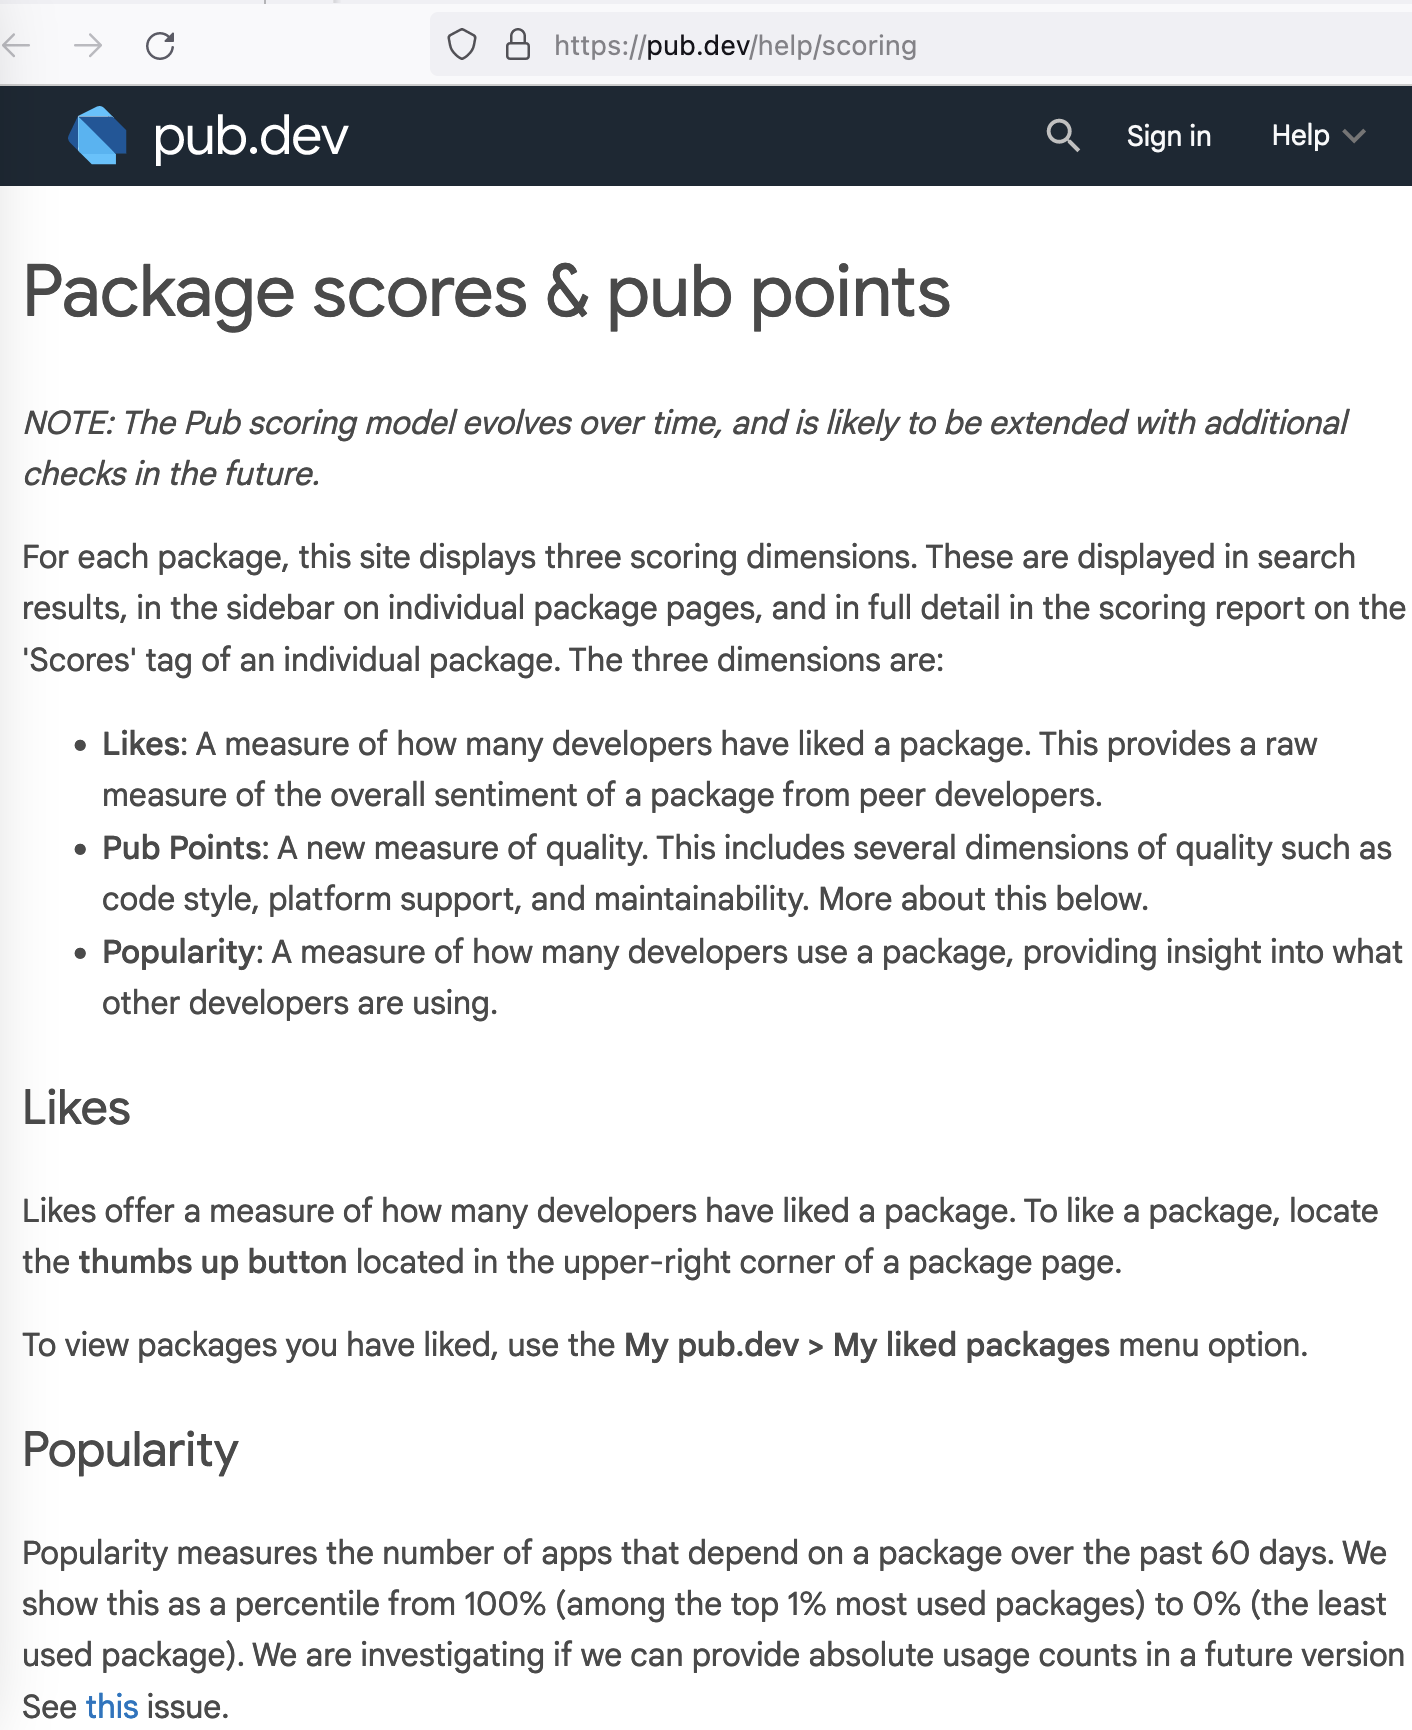
\includegraphics[width=30em]{pub-scoring}
\end{center}

\pagebreak
